\documentclass[a4paper,11pt]{report}
\usepackage[T1]{fontenc}
\usepackage[utf8]{inputenc}
\usepackage{lmodern}
\usepackage[francais]{babel}
\usepackage{graphicx}
\usepackage{array}

\title{}
\author{}

\begin{document}

\maketitle
\tableofcontents

\begin{abstract}
\end{abstract}

\chapter{Partie reseau}

\section{Modélisation des classes de réseau}

    \begin{figure}[th]
      \begin{center}
        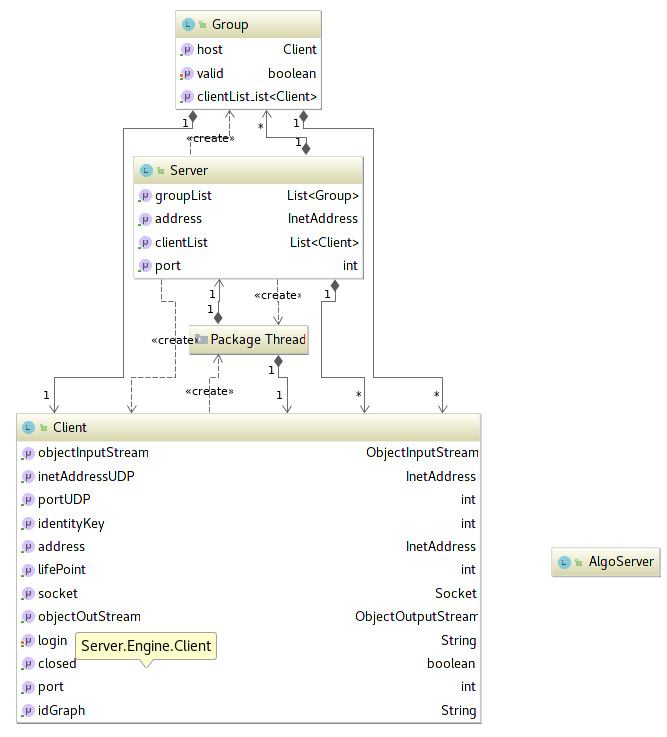
\includegraphics[scale=0.6]{Assets/UML_serveur.png}
        \caption{UML du serveur}
        \label{UML du serveur}
      \end{center}
    \end{figure}
    
    Le serveur contient des clients et des groupes et les groupes contiennent eux même des clients.
Un groupe possède en variable d’instance son hôte. 
Un client possède les flux objets, son socket et ses coordonnées pour le transport UDP.
Et le serveur son socket serveur TCP et UDP.



\subsection{UML de gestion des clients pour le serveur}

\subsection{UML de gestion des données pour les clients}


\section{Modélisation des classes de réseau}



\section{Les classes annexes}

\end{document}
